\section{L'ambiente di sviluppo}



\subsection{Tensorflow}
Naturalmente la progettazione di una rete neurale per l’apprendimento automatico è un lavoro lungo e argusto;
freamework come Theano, Torch o Tensorflow  rendono la generazione delle reti neurali un lavoro più semplice e piacevole offrendo allo sviluppatore tutto un set di metodi e modelli già implementati e largamente testati.
Per questo progetto è stato scelto Tensorflow sicuramente il più peculiare,vasto ed adattabile.
questa adattabilita è possibile  grazie al fatto che tutto il progetto è open source è infatti rilasicato da Google con licenza Apache 2.0 e dalla attiva comunity che vi è dietro.Le librerie di Tensorflow sono  disponibili in diversi linguaggi tra cui i piu annoverati sono Java,C,C++ e Python , quest' ultimo è stato scelto per questo progetto,nonostante gran parte del sorgente sia in c++ in quanto più agevole all' interno della suite di sviluppo di Google Collab(che introdurrò in seguito).i modelli creati con tensorflow possono essere addestrati sia svolgendo i calcoli su cpu che sfruttando l'accellerazione su gpu con le varie implementazioni di cudNN( per schede Nvidia utilizza i core CUDA  per offrire prestazioni superiori) e ROCM(che permette l'esecuzione anche su schede amd  )

\subsection{OpenCv}
Open Cv è una libreria software che si rileva essere essenziale quando si vuole lavorare con le immagini sopratutto in un AttnGAN in quanto rende possibile il riconoscimento delle parti dell'immagine e tutta una serie di trasformazioni morfologiche di quest'ultime ; è rilasciata sotto licenza BSD 




\subsection{Google Collab}
Durante l'addestramento sono state utilizzate diverse macchine , i primi test su un normale portatile in ambiente linux,poi l'addestramento in un container docker utilizzando due schede AMD e i driver ROCM, ed infine il cloud computing offerto da Google Collab con il quale sono stati ottenuti i risultati migliori ,ho ritenuto giusto di conseguenza soffermarmi solamente su quest' ultimo.

Google Collab è sostanzialmente un servizio che permette l'accesso ad un server virtuale sul quale è possibile eseguire qualunque tipo di progetto di Deep learning  ; la modalita di accesso è simile all'ssh(seppur in maniera  molto più limitata)abbiamo davanti a noi una sorta di terminale bash interattivo ,  il tutto è condito con con una serie di tool che permettono l'accesso ai dati salvati sul drive di Google  e la creazione di un cosi detto "Jupyter Notebook" cioè di una serie di comandi (potremmo dire script) da eseguire per avviare le varie procedure di training e di monitoraggio  che possono essere condite di testo ed immagini per clarificare le operazioni;si può segliere poi il linguaggio di runtime desiderato e iniziare la procedura il tutto comodamente dalla schermata del proprio browser preferito \\
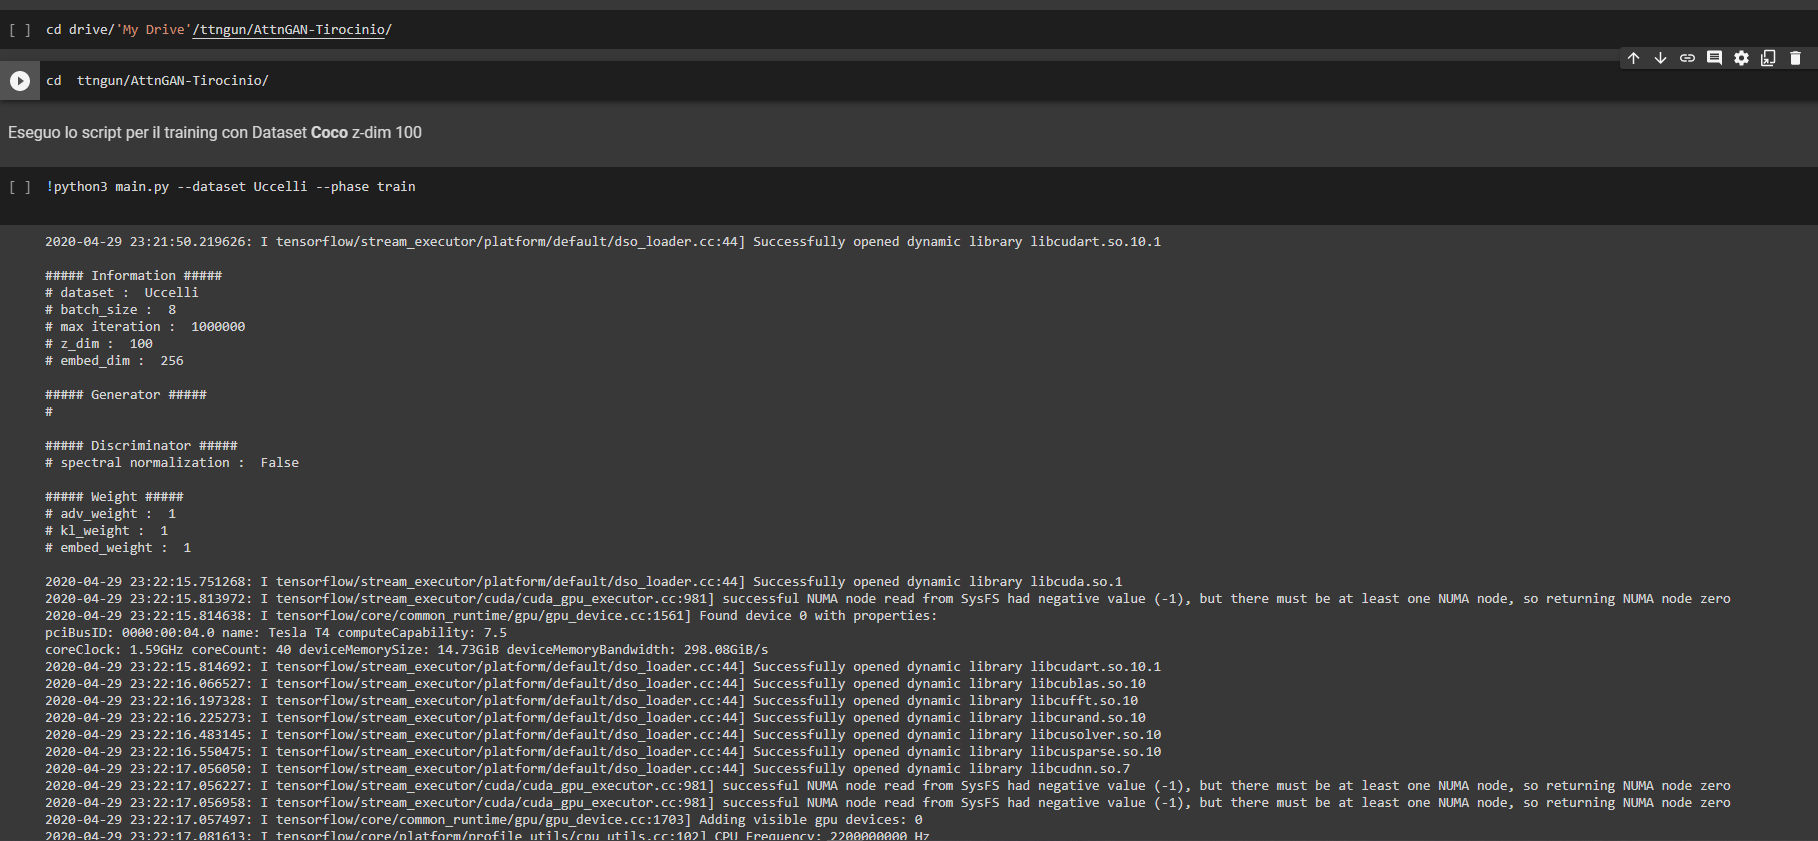
\includegraphics[scale=0.3]{collab}



\subsection{Python}


Python nato nel 1991 è un linguaggio multiparadigma fortemente tipato. 
Le sue peculiarità sono la flessibilità del codice e le numerose piattaforme su cui gira, visto che il codice viene compilato ed eseguito su una macchina virtuale.Python è famoso per essere il linguaggio più utilizato  nel mondo dell’intelligenza artificiale ed è quindi adattissimo per iniziare vista la quantita di materiale reperibile in rete. Dei freamework  specializzati in questo ambito la stragrande maggioranza è compatibile o addirittura è "madre lingua ;i primi sviluppatori e ricercatori in questo ambiente infatti hanno trovato la sua semplicità d' uso come un punto di forza ;per quanto concerne le prestazioni tutta via ,nonostante i miglioramenti negli ultimi anni, i risultati sono molto inferiori a quelle che linguaggi meno astratti come il C++ possono ottenere;per ridurre i tempi di esecuzione la macchina virtuale usa una strategia di caching aggressiva ma naturalmente tutto ciò è solo una mitigazione del problema.Grande punto di forza di questo linguaggio è l'ottimizzazione per il lavoro con le matrici che sono naturalmente essenziali quando si elaborano reti neurali o più in generale grafi pesati di qualunque genere le librerie più importanti per il calcolo matriciale e la gestione delle matrici sono Pymatrix e Numpy(di cui faccio largamente uso nel progetto).Anche per Python naturalmente la comunity di utilizzatori è molto vasta e questo permette di risolvere la maggior parte dei problemi con una ricerca online .


\subsection{Dataset}
Il dataset è l'insieme di tutti quei dati che consideriamo reali e validi  sul quale la rete discriminatrice si basa per calcolare la veridicità di un dato;
il Dataset non è quindi nient altro che una raccolta di esempi organizzati in maniera che siano comprensibili per il disriminatore.Il sistema impara quindi a "conoscere" le differenze e le somiglianze tra tutti gli esempi.
Prendiamo come esempio un sistema che generi dei fiori il dataset sara formato da il maggior numero possibile di foto di  fiori che differiscano il minimo possibile nei dettagli che non ci interessano ;naturalemente in realta ci sara sempre una differenza "ambientale" tra le varie foto ,tuttavia se si mantiene un certo contesto tutto questo risulta accettabile.In questo progetto prenderemo in esame il database CUB-200-2011 della Caltek che altro non è che una raccolta di foto di volatili tutti classificati per nome.
\begin{figure}[h]
\caption{Foto presenti in Cub-200-2001}
\centering
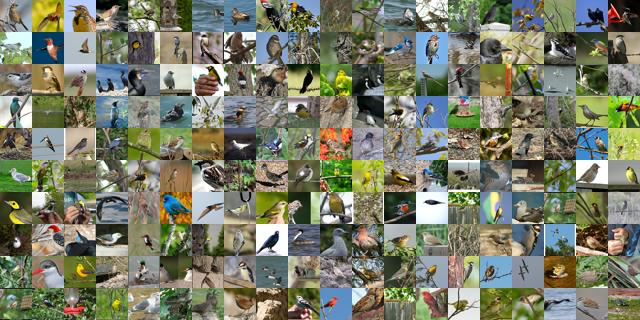
\includegraphics[scale=0.5]{collage} 
\end{figure}
\\
Date le specifiche  del progetto abbiamo anche bisogno di una descrizione per ogni immagine ,quindi un file di testo che contiene un identificativo dell'immagine di riferimento ,in realta per ottenere una rete generativa che esuli da uno specifico ordine delle parole e sia il più possibile linguisticamente completa abbiamo bisogno di diversi testi descrittivi per ogni singola immagine  cosi come di diverse immaggini per ogni singolo volatile; è proprio l'insieme di queste due caratteristiche che rende come prima detto l'ambiente circostante al caso di studio il meno incidente possibile .
Per massimizzare le probabilità di riuscita e la qualità dei risultati è molto importante infatti  fornire un dataset di soggetti specifici  e di vaste dimensioni. Per migliorare la qualità degli esempi forniti in input al sistema è necessario riuscire ad offrire un numero di elementi il più possibile rassomiglianti tra di loro, in modo che il processo di apprendimento risulti il più veloce possibile poiché riconoscere somiglianze e pattner sarà più semplice per il calcolatore; in sostanza infatti possiamo dire che più un dataset è specifico piu è veloce l'apprendimento e migliori sono i risultati
\subsection{Il loop di apprendimento }
Scrivere il codice della Gan è solo una frazione del lavoro svolto  molto più lungo infatti è il processo di addestramento e la ricerca di tutti quei parametri dimensionali ,tra cui la dimensione dell'immagine in output che permettono alla gan addestrata di creare un dato plausibile.




Fortunatamente durante l’esecuzione dell’applicazione è possibile usufruire di determinate informazioni che renderanno più semplice comprendere in quale direzione l’allenamento sta andando, e con una discreta quantità di nozioni è possibile individuare eventualmente le cause di fallimento del sistema. C’è da dire in ogni caso che studiare gli output è già di per sé uno strumento di analisi molto potente nel caso di malfunzionamenti. In effetti la più grande difficoltà della curva di apprensione di questa tecnologia è quella di riuscire ad interpretare i dati che vengono forniti dal sistema per trovare un equilibrio nel ciclo allo scopo di rendere le due reti neurali equilibrate in quanto a capacità. 
In questo caso specifico, il generatore procederà per tentativi cercando di fare il “passo corretto” volta per volta fino a riuscire a beffare l’altra rete, mentre il discriminatore dovrà scegliere il suo output in relazione al suo livello di allenamento che aumenterà di epoca in epoca (per “epoca” si intende ciclo di allenamento). A questo punto pensare che sarà più semplice per il discriminatore scegliere piuttosto che per il generatore trovare una via corretta viene da sé, e questo comporta una serie di problematiche che dovranno essere affrontate nella maniera più corretta possibile. In questo capitolo verranno analizzati i comportamenti delle due reti al crescere della lunghezza dell’allenamento e verranno proposte delle soluzioni ai problemi più comuni che vengono incontrati durante l’allenamento di questo tipo di reti neurali. 
